%============================================================
% 6. 交通
%============================================================
\section{交通}\label{sec:traffic}

\subsection{哥本哈根公共交通介绍}

\subsubsection{巴士}
遍布整个首都地区，贯穿哥哈城区的主要交通方式之一。可在巴士上向司机购买单程票，或提前在车站自动售卖机与线上 APP 购买车票。站台及 APP 可实时查看到站时间。

\subsubsection{地铁}
主要覆盖市中心／机场（1–4 区）。\textbf{必须在上车前持有有效车票}；四条线路 \texttt{M1\textendash M4}。详见官网：
\url{https://www.m.dk/rejser/se-metroens-linjer/}

\subsubsection{城郊火车（S-tog）}
遍布首都大区，以字母+终点站区分线路。\textbf{上车前须持票}。线路图：
\url{https://www.dsb.dk/s-tog/}

\subsubsection{城际火车（regional tog）}
连接丹麦主要城市，现场或线上购票：
\url{https://www.dsb.dk/}

\subsubsection{黄色火车（Lokaltog）}
服务哥本哈根地区：\url{https://www.lokaltog.dk}

\subsubsection{轻轨（建设中）}
预计 2025 年通车，Lyngby–Ishøj 方向：
\url{https://www.dinletbane.dk}

%------------------------------------------------------------
\subsection{交通卡 \textit{Rejsekort} 办理}\label{sec:rejsekort}

\begin{itemize}[leftmargin=1.5em]
  \item 线下机可办\textbf{匿名卡}（70 DKK），线上/APP 办\textbf{实名卡}（20 DKK）。
  \item 乘车前 \textit{Check-in}，下车 \textit{Check-out}，按区数计费；比单程票便宜（单程最低 24 DKK）。
  \item 卡片类型  
        \begin{itemize}
            \item \textbf{实名卡}：仅本人使用，优惠最大，可邮寄到家；  
            \item \textbf{匿名／灵活匿名卡}：后者可借他人且享一定优惠，可官网下单。
        \end{itemize}
\end{itemize}

\begin{figure}[htbp]
    \centering
    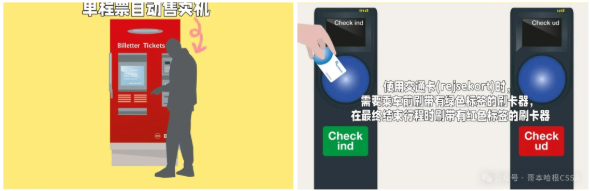
\includegraphics[width=.9\linewidth]{figures/rejsekort_machine.png}
    \caption{单程票售票机与 Rejsekort 打卡示意}
\end{figure}

%------------------------------------------------------------
\subsection{交通 APP}\label{sec:traffic-app}

\begin{figure}[htbp]
    \centering
    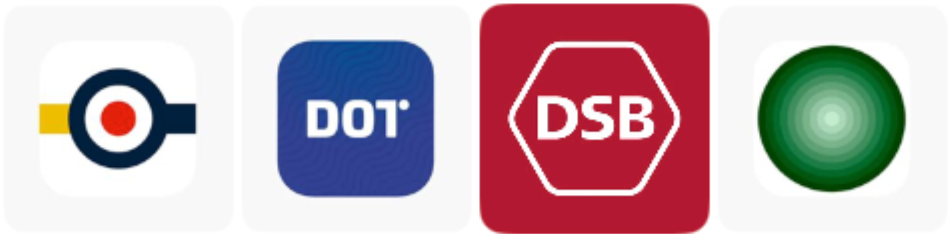
\includegraphics[width=.7\linewidth]{figures/transport_apps.png}
    \caption{常见公共交通 APP（左起：Rejseplanen、DSB、DOT、RejseBillet）}
\end{figure}

\subsubsection{Rejseplanen}
查询全部公共交通线路与实时到站／延误。

\subsubsection{DOT}
购单程票、月票、通勤卡，激活青年卡。

\subsubsection{DSB}
城际火车购票；支持月票、往返瑞典南部月票等。

\begin{grayleftbox}
\textbf{学长学姐碎碎念 }
\begin{itemize}
  \item 我拥护 DSB!!，非高峰自带折扣，信用卡协议免验证。购票或充值可获 7-11 积分，免费兑换吃喝。
\end{itemize}
\end{grayleftbox}

\subsubsection{RejseBillet}
2023 新 APP，与 DOT 功能重叠，未来可能整合。

%============================================================
% 7. 购物
%============================================================
\section{消费 \& 购物}

\subsection{二手交易平台}
\begin{itemize}
  \item \textbf{DBA}
  \item \textbf{Facebook Marketplace}
  \item \textbf{微信群}
\end{itemize}

\subsection{日常消费App推荐}
\begin{itemize}
  \item \textbf{MineTilbud} — 超市打折聚合 APP  
  \item \textbf{Lidl Plus} — 会员折扣+积分  
  \item \textbf{Netto+ Scan \& Go} — 免排队、免国内卡手续费  
  \item \textbf{Too Good To Go} — 盲盒 app，冬天囤早餐食材
\end{itemize}

% ============================================
% chapters/bank_cards.tex
% 银行卡主流选项对比（层级统一下调版）
% ============================================

% --------------------
% Subsection: 银行卡主流选项对比
% --------------------
\subsection{银行卡}

% --------------------
% Subsubsection: 关键办理要点
% --------------------
\subsubsection{关键办理要点}

\begin{enumerate}[leftmargin=3em,label=\arabic*.]
  \item \textbf{必备文件}\\
        护照、丹麦 CPR 号（黄卡）、居留许可、MitID 是所有银行通用硬指标。线上或线下银行均可能核对这些信息。
  
  \item \textbf{开户速度}\\
        \textbf{Revolut/Lunar}：视频或自拍认证后即刻得到虚拟卡，实体卡 3–7 天寄达。\\
        \textbf{传统银行}：在线申请 → 邮件/电话排队 → 线下面谈（约 30 min）→ 等待后台审批，整体 1–4 周不等。
  
  \item \textbf{费用 \& 账户维护}\\
        学生套餐多为 0 DKK/月，但超过年龄／毕业后可能转为普通账户；少数银行会收取季度费。使用前确认收费及变更条款。
  
  \item \textbf{多币种与外汇}\\
        \textbf{Revolut}：36 种即时汇兑，适合从人民币汇款兑换 DKK。\\
        \textbf{Lunar/Danske} 等本地银行多币功能有限，跨境电汇手续费 50–75 DKK 起。
\end{enumerate}

% 银行对比表
\subsubsection{留学生部分常见银行卡对比}
\begin{table}[H]
  \scriptsize
  \rowcolors{2}{gray!10}{white}
  \centering
  %\caption{中国}
  \label{tab:bank_compare_new}
  \renewcommand{\arraystretch}{1.25}
  \setlength{\tabcolsep}{5pt}
  \begin{tabularx}{\textwidth}{p{0.12\textwidth} p{0.09\textwidth} p{0.13\textwidth} p{0.15\textwidth} X X}
    \toprule
    \textbf{银行/账户} & \textbf{是否线上} & \textbf{NemKonto 支持} & \textbf{学生/青年费用} & \textbf{主要优势} & \textbf{主要限制} \\
    \midrule
    Revolut & \cmark 全 App & \xmark\ 无法直接设为 NemKonto（需本地银行） & 标准版 0 DKK/月 & 开户秒批、36 币种、国际汇兑手续费低 & 仅电子卡/英欧 IBAN \\
    Lunar（Luna Bank） & \cmark 全 App & \warn\ 手续比传统银行多 & Lunar Standard 0 DKK/月 & 快速开户、英文界面、实体+虚拟卡任选 & 仍需 CPR + MitID；无线下网点 \\
    Lån \& Spar（配合 IDA/Djøf 工会） & \xmark 需到店 & \cmark  & 0 DKK/月；活期利率高 5\% & 与工会合作，手续简易，利率高 & 需成为 IDA/Djøf 成员；线下面谈一次 \\
    Danske Bank & 部分线上 & \cmark & 18–27 岁或 ≤32 岁学生：0 DKK/月（含 2 账户+2 卡） & 丹麦最大银行，英文 App 全功能 & 等待开户 2–4 周 \\
    Sydbank & 部分线上 & \cmark & 18–29 岁：账户及 Visa/Mastercard 免年费 & 客户服务口碑好，可免费 ISIC 学生卡 & 服务网点少；非学生套餐收费高 \\
    Nordea & 部分线上 & \cmark & 官方 Mobile Plus 套餐 0 DKK/月；部分分行学生卡约 90 DKK/季 & 可申请 Nordea Gold 信用卡（含旅行险），含信用额度上限 2 000 € & 免费套餐需先开 Mobile Plus；信用额度审批较严 \\
    \bottomrule
  \end{tabularx}
\end{table}

% 灰条提示框：阅读指南
\begin{grayleftbox}
\small
\textbf{表格阅读指南: }
\begin{itemize}
  \item \textbf{“纯线上"}：开户全过程均在 App／网页完成，可立即拿到虚拟卡。如需实体卡邮寄到丹麦地址。
  
  \item \textbf{“部分线上"}：申请表在网上填写，但由于反洗钱法规（AML/KYC）仍必须做一次身份核验，方式通常有
    \begin{enumerate}[leftmargin=2em,label=\arabic*.]
      \item 到指定网点或快闪柜台 (pop-up) 面对面验证护照 + CPR + 居留卡；
      \item 通过视频通话上传护照 + 自拍（身份核对法）。只有完成这一步，账户才会激活并能设为 NemKonto。
    \end{enumerate}
\end{itemize}
\end{grayleftbox}

% 灰条提示框：办理小贴士
\begin{grayleftbox}
\textbf{办理小贴士: }
\begin{itemize}
  \item 入学高峰银行排队久，线上申请可抢进度；线下面谈务必带护照、黄卡、居留卡原件。
  \item 在校期间充分利用学生免费套餐和福利；毕业或超龄后及时评估转账/关户成本。
\end{itemize}
\end{grayleftbox}


%============================================================
% 8. 医疗 & 保险
%============================================================
\section{医疗 \& 保险}

\subsection{哥本哈根公共医疗简要说明}
持 \textbf{黄卡 (Sundhedskort)} 可享免费公共医疗。黄卡=CPR + 国家医保，涵盖 GP、急诊室、住院等（牙科、处方药、心理治疗大多需自费或部分补贴）。

\subsubsection{非紧急情况}
\begin{enumerate}
  \item 家庭医生 (\textbf{GP})：慢性病、感冒等  
  \item 专科：GP 转介后就诊（耳鼻喉科可直挂）  
  \item 夜间急诊：拨 \textbf{1813}
\end{enumerate}

\subsubsection{紧急情况}
\textbf{112} — 生命危险立即呼救。任何生命危险或重大创伤（心脏骤停、严重交通事故等）直接 112。

\subsubsection{心理辅导}\label{sec:mental-emergency}

\begin{table}[htbp]
  \small
  \rowcolors{2}{gray!10}{white}
  \centering
  \setlength{\tabcolsep}{6pt}
  %\caption{}
  \begin{tabularx}{\textwidth}{X l}
    \toprule
    \textbf{哥本哈根 24h 心理急诊地址} & \textbf{热线} \\
    \midrule
    Digevej 110, 2300 København S                & 38 64 16 50 \\
    Maglevænget 2, 2750 Ballerup                 & 38 64 50 03 \\
    Esther Ammundsens Vej 36A, 2400 København NV & 38 64 73 60 \\
    \bottomrule
  \end{tabularx}
\end{table}

\begin{grayleftbox}\textbf{小贴士:}
1813 覆盖整个首都大区，24 小时可拨打。工作日 08 – 16 点应优先联系自己的 GP；其余时段（夜间、周末、节假日）或 GP 无法接通时，再拨 1813。
\end{grayleftbox}

%------------ 就医 APP 表格 -----------------
\subsection{就医 APP 介绍}
\begin{itemize}
  \item \textbf{Min læge} — 线上问诊、预约、查询记录
  \item \textbf{Sundhedskortet} — 电子黄卡
  \item \textbf{Min sundhed} — 查询记录、疫苗证明
\end{itemize}

\begin{grayleftbox}\textbf{常用药物小 Tips:}
丹麦处方药管制严格，下列常用药仅凭处方购买：抗生素、肠胃药、感冒/退烧药、慢性病药、中成药。
\end{grayleftbox}



%============================================================
% 10. 手机卡 & 宽带套餐
%============================================================
% \section{手机卡 \& 宽带套餐}

% \begin{grayleftbox}{个人经历}
% 下飞机后地铁站免费领取 \textbf{Lyca} 卡，插卡即用。APP 购买套餐有优惠，流量马上生效。
% \end{grayleftbox}


% ---------- End of code ----------
